\chapter{Methodology}
\label{chap:methodology}

\section{Overview of the Methodology}

This chapter describes the methodological framework developed to optimize the operational costs of Water Supply Systems (WSS) through the integration of the DC3 (Deep Constraint Completion and Correction) algorithm with the duty-cycle formulation. 

The proposed method extends the approach presented on article Cost efficiency in water supply systems: An applied review on optimization models for the pump scheduling problem \cite{rfc20}, in which three optimization formulations were compared: binary genetic algorithm (B-GA), real-continuous sequential least squares programming (RC-SLSQP), and duty-cycle sequential least squares programming (DC-SLSQP). While the DC-SLSQP approach already allows for greater flexibility in pump scheduling by considering continuous start and duration times for each duty cycle, the present work enhances it through a deep learning model capable of learning feasible and near-optimal solutions under nonlinear hard constraints.


\subsection{The DC3 Algorithm}

The DC3 algorithm\cite{rfc14}, introduces a two-stage learning mechanism for constrained optimisation:
\begin{enumerate}
    \item \textbf{Constraint Completion:} infeasible points are projected into the feasible subspace defined by the equality constraints.
    \item \textbf{Constraint Correction:} feasible points are further adjusted to satisfy inequality constraints.
\end{enumerate}

DC3 guarantees that the network outputs remain within feasible regions, even when trained on incomplete or noisy data. Its differentiable projection operators make it particularly suitable for complex systems such as WSS, where physical feasibility (e.g., hydraulic balance) must be maintained at all times.

\section{Illustrative Example: Nonlinear Constrained Optimisation Problem}

To demonstrate the operation of the DC3 algorithm, a simple nonlinear optimisation problem with one equality and one inequality constraint was implemented as a conceptual test case \cite{rfc21}. This example precedes the full-scale water supply optimisation presented in Chapter~\ref{chap:methodology}.

\begin{equation}
\begin{aligned}
\min_{x_1, x_2} \quad & f(x_1, x_2) = x_1 \big((x_1 - x_2)^2 + (x_1 - 2)\big) + 5, \\
\text{s.t.} \quad & h(x_1, x_2) = \tfrac{1}{2}x_1^2 + 1.5x_2^2 - 1.2 = 0, \\
& g(x_1, x_2) = 0.75x_1^2 + 0.25x_2^2 - 0.5 \le 0.
\end{aligned}
\end{equation}

The equality constraint defines an elliptical curve in the $(x_1, x_2)$ plane, while the inequality constraint delimits an elliptical feasible region. The DC3 mechanism is used to project infeasible points into this feasible region while ensuring that the equality constraint remains satisfied.

\begin{figure}[H]
    \centering
    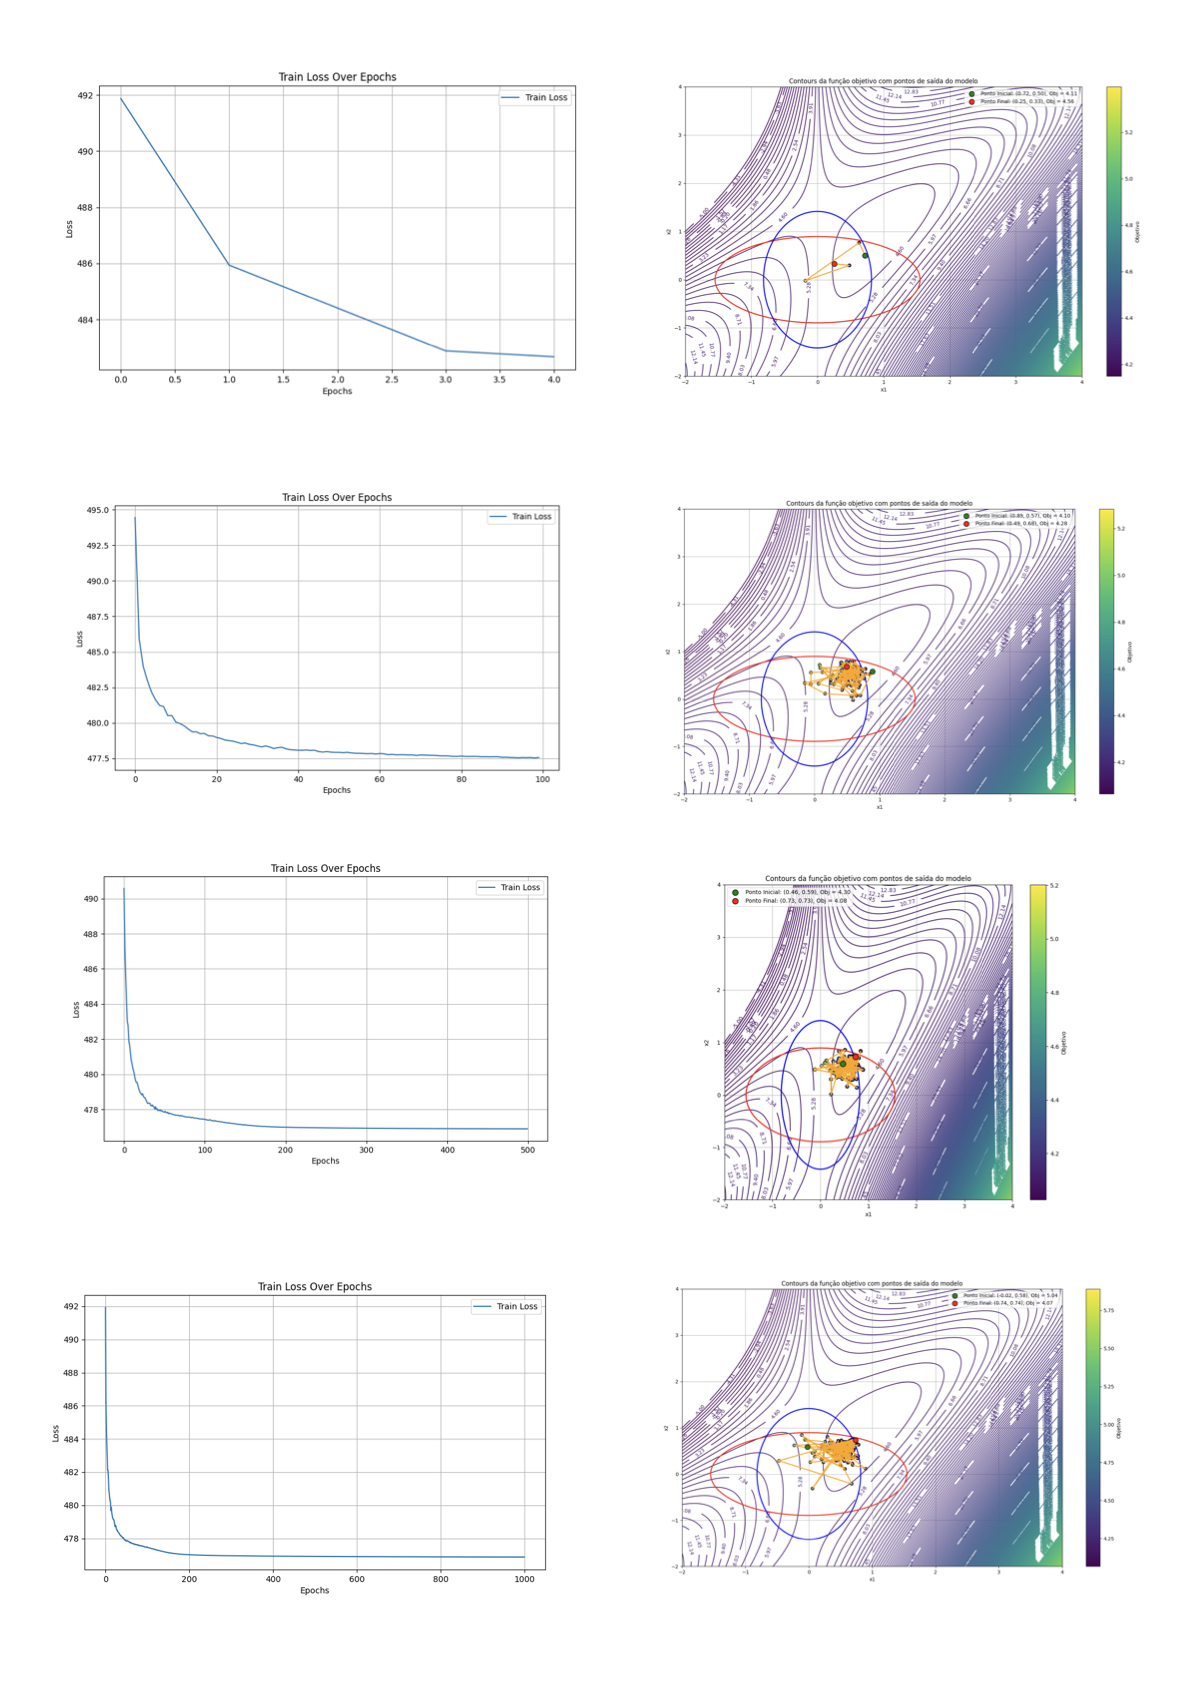
\includegraphics[width=0.7\textwidth]{figs/nonlinear_problem.jpeg}
    \caption{Illustrative nonlinear constrained optimisation problem showing the feasible region (blue), equality constraint $h(x)=0$ (red dashed line), and inequality boundary $g(x)=0$ (blue solid line).}
    \label{figs:nonlinear_problem}
\end{figure}

This example demonstrates DC3’s ability to perform both \textit{constraint completion} and \textit{constraint correction}, maintaining feasibility throughout the optimisation process. The concepts validated in this example are extended to the water supply optimisation case studies in the next chapter.


\section{Problem Formulation for Water Supply Systems}

The optimization problem aims to minimize the total energy cost of pump operation over a 24-hour time horizon. Following Brás et al. (2023), the formulation considers the operational constraints of the system, including water tank levels, pump operating limits, and time-dependent energy tariffs.

The duty-cycle formulation defines, for each pump, two sets of decision variables:
\begin{itemize}
    \item $x_{p,d}^{start}$ – start time of duty-cycle $d$ for pump $p$;
    \item $x_{p,d}^{dur}$ – duration of duty-cycle $d$.
\end{itemize}

The optimization model can be expressed as:

\begin{equation}
\begin{aligned}
\min_{\mathbf{X}_{dc}} \quad & C(\mathbf{X}_{dc}) = 
\sum_{p=1}^{P} \sum_{d=1}^{D} \frac{1}{\eta_p} \, W_p(x_{p,d}) \, \tau(x_{p,d}) \, x_{p,d}^{dur} \\
\text{s.t.} \quad & h_{min} \leq g_t(\mathbf{X}_{dc}) \leq h_{max}, \\
& t_{min} \leq x_{p,d}^{start} \leq t_{max}, \\
& x_{p,d+1}^{start} \geq x_{p,d}^{start} + x_{p,d}^{dur}, \\
& g_{temp\_log}(\mathbf{X}_{dc}) \leq 0.
\end{aligned}
\end{equation}

where $C(\mathbf{X}_{dc})$ is the total energy cost, $\tau$ the time-dependent tariff, $\eta_p$ the pump efficiency, and $g_t$ the hydraulic behavior evaluated by the WSS predictor (based on EPANET simulations). 

The system constraints ensure that the tank levels remain within admissible limits ($h_{min}$, $h_{max}$), the duty cycles do not overlap, and all operations respect temporal boundaries.

\section{DC3-Based Optimization Framework}

To handle the nonlinear and hard constraints of this problem, the DC3 learning framework was integrated with the duty-cycle formulation. The class \texttt{Problem\_DC\_WSS} defines all components required for the DC3 training process:
\begin{itemize}
    \item The objective function (\texttt{obj\_fn\_Autograd}) computes the total operational cost, incorporating differentiable autograd operators.
    \item The inequality residuals (\texttt{ineq\_resid\_autograd}) represent the constraint violations for tank levels, pump timing, and temperature log conditions.
    \item The function \texttt{ineq\_dist\_autograd} computes the ReLU-based clamped distances to ensure differentiability of the hard constraints.
    \item The Jacobian functions (\texttt{jac\_gT\_Original}, \texttt{jac\_TempLog\_Original}, and \texttt{jac\_x\_Autograd}) define the gradient structure used by DC3 for constraint correction.
\end{itemize}

The network learns feasible mappings between input data (system demand patterns and decision variables $\mathbf{y}$ that minimize the cost while maintaining hydraulic feasibility.

The \texttt{process\_output\_original} and parametric variants (1–3) implement differentiable mappings that convert raw network outputs into valid pump schedules. These mappings ensure:
\begin{enumerate}
    \item Non-overlapping start times for duty cycles;
    \item Durations within the range $[0.001, 5.0]$ hours;
    \item Adjustment of end times to remain within the daily horizon $[0, 23.9]$ hours.
\end{enumerate}

\section{Model Training and Implementation}

The DC3-based optimization model is implemented in Python using PyTorch for automatic differentiation and neural network training.

In this study, we use 100 examples of pump duty cycles, constructed under the constraint criteria, to train and warm-start the model. These examples feature varied start and end times while always respecting the limit of five daily duty cycles per pump. To ensure feasibility and diversity, start–duration pairs are sampled within the daily horizon and then projected through the differentiable post-processing mappings (\texttt{process\_output\_original} and its parametric variants) to enforce: (i) non-overlapping cycles, (ii) durations within $[0.001, 5.0]$ hours, and (iii) end times clipped to $[0, 23.9]$ hours. Each candidate schedule is validated with the WSS predictor (EPANET-based); infeasible samples are rejected. The final set covers multiple tariff periods and demand regimes to improve generalization. We use these 100 feasible schedules to bootstrap learning via a short supervised pretraining phase (e.g., minimizing a Huber/MSE loss between network outputs and seed schedules for a few epochs) before switching to the full DC3 objective. During subsequent training, seed samples are interleaved in mini-batches to stabilize learning and reduce early constraint violations.

The training process is implemented in the \texttt{train\_net()} routine. The model is trained over the available demand data divided into training, validation, and test sets according to the proportions $83.3\%$, $8.3\%$, and $8.3\%$, respectively.

During each epoch, the solver network (\texttt{NNSolver}) predicts an initial solution $\hat{Y}$, which is refined through gradient-based correction steps using the DC3 update rule:
\[
Y_{new} = \hat{Y} - \alpha \, \nabla L_{ineq}(Y),
\]
where $L_{ineq}$ is the inequality constraint loss computed from \texttt{ineq\_dist\_autograd} and $\alpha$ is the learning rate.

The training objective combines the total operational cost with a soft penalty on constraint violations:
\[
L_{total} = L_{obj} + \lambda (1 - \lambda_{eq}) L_{ineq},
\]
where $L_{obj}$ is the energy cost, and $\lambda$ regulates the balance between cost minimization and constraint enforcement.


The optimization of network weights is performed using the Adam optimizer, with learning rate $\texttt{lr}$ and batch size $\texttt{batchSize}$. Visualization tools are employed to monitor the tank level evolution, pump operations, and inequality distances throughout training epochs, ensuring convergence toward feasible and efficient operational schedules.

